\subsection{Ejercicio 3}

Para realizar la tarea TaskBatch se generaron cant_bloqueos números distintos aleatoriamente dentro del rango [0, total_cpu -1]. Al hacerlo se tuvo en cuenta el hecho de que se pueden obtener números repetidos.
Luego, si el momento coincidia con el número generado al azar, se llamaba a la funcion que simula los bloqueos (uso_IO).

La tarea generada es la siguiente

\begin{figure}[h]
  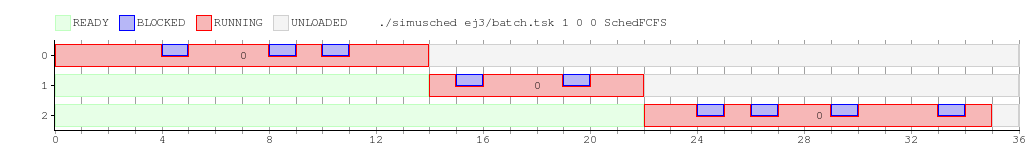
\includegraphics[width=\textwidth]{../ej3/salida.png}
  \caption{}
\end{figure}
